\documentclass[12pt,a4paper]{article}

% Packages
\usepackage{amsmath,amssymb,amsfonts}
\usepackage{tikz}
\usepackage{graphicx}
\usepackage[margin=1in]{geometry}
\usepackage{hyperref}
\usepackage{enumitem}
\usepackage{tcolorbox}
\usepackage{fancyhdr}
\setlength{\headheight}{15pt}


% Header and footer
\pagestyle{fancy}
\fancyhf{}
\rhead{MATH 311}
\lhead{Vedant Patil}
\cfoot{\thepage}

% Title
\title{Lecture Notes: Section 2.3}
\author{Vedant Patil}
\date{\today}

\begin{document}

\maketitle

\section{Overview}
\begin{tcolorbox}[colback=yellow!10!white,colframe=yellow!50!black,title=Key Points]
  \begin{itemize}
    \item Set Notation 
    \item Operations on Sets
    \item Distributive and DeMorgan's Laws
  \end{itemize}
\end{tcolorbox}

\section{Detailed Notes}
\subsection{Set Notation}
We write sets with noation as follows \\ 
\begin{equation}
  \{a_{1},a_{2},a_{3},a_{4},a_{5}\}
\end{equation}
This is a set with 5 elements and there doesn't have to be any relation with the elements 
\begin{equation}
  \{ \text{apple, 5, blue}, -\frac{1}{2}\}
\end{equation}
This is a example of a set wtih 4 elements that have no relation to each other 
\\ 
We might sometimes let \( \mathbb{S} \) denoate a universal set of everything we are considering 
\begin{equation}
  A \subseteqq B \text{ or} A \subset B \text{ means A is a subset of B} 
\end{equation}

Null set notation 
\begin{equation}
  \emptyset \text{ is a empty set. The empty set has no elements }
\end{equation}

\begin{equation}
  \text{For any set A, the empty set is a subset of A} \emptyset \subseteqq A 
\end{equation}

\subsection{Operations on Sets}
If A and B are sets we are going to make some other sets 

\hspace{3pt}

Union 
\begin{equation}
  A \cup B \text{ is a set of everything that is in A or B}
\end{equation}

\begin{center}
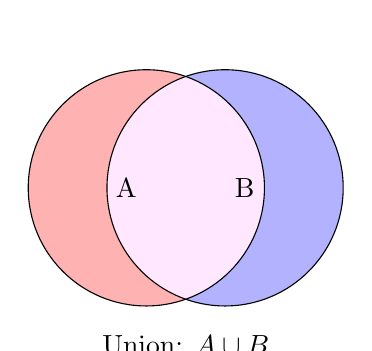
\begin{tikzpicture}
  \begin{scope}[blend mode=screen]
    \fill[red!30] (0,0) circle (1.5);
    \fill[blue!30] (1,0) circle (1.5);
  \end{scope}
  \draw (0,0) circle (1.5) node [left] {A};
  \draw (1,0) circle (1.5) node [right] {B};
  \node at (0.5,-2) {Union: $A \cup B$};
\end{tikzpicture}
\end{center}

Intersection 
\begin{equation}
  A \cap B \text{ is a set of everything that is in A and B}
\end{equation}

\begin{center}
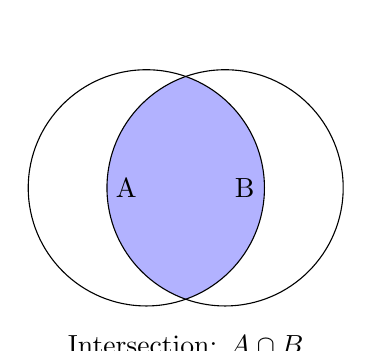
\begin{tikzpicture}
  \begin{scope}
    \clip (0,0) circle (1.5);
    \fill[blue!30] (1,0) circle (1.5);
  \end{scope}
  \draw (0,0) circle (1.5) node [left] {A};
  \draw (1,0) circle (1.5) node [right] {B};
  \node at (0.5,-2) {Intersection: $A \cap B$};
\end{tikzpicture}
\end{center}

The compliment of a Set A is \( \overline{A} \)
\begin{equation}
  A \in \overline{A} \text{ means} x \notin A (\text{x is not in A})
\end{equation}

Two sets are disjoin or mutually exclusive if \(  A \cap B = \emptyset \)


\section{Important Formulas/Theorems/Definitions}
\begin{tcolorbox}[colback=blue!5!white,colframe=blue!75!black,title=Key Formula/Theorem]
  DeMorgan and Distributive Laws 
  \begin{equation}
    A \cap (B \cup C) = (A \cap B) \cup (A \cap C) 
  \end{equation}
  \begin{equation}
    A \cup (B \cap C) = (A \cup B) \cap (A \cup C)
  \end{equation}
  \begin{equation}
    \overline{(A \cap B)} = \overline{A} \cup \overline{B}
  \end{equation}
  \begin{equation}
    \overline{(A \cup B)} = \overline{A} \cap \overline{B}
  \end{equation}
\end{tcolorbox}

\section{Examples}
\begin{tcolorbox}
  Flip a coin twice 
  \begin{equation}
    s = \{ HH, HT, TT\}
  \end{equation}
  \begin{equation}
    \text{Let } A = \{HH, HT\}, \text{ the set of outcomes with heads on the first flip}
  \end{equation}
  \begin{equation}
  B = \{ HH, TT\} \text{ the set of outcomes where both flips are the same}  
  \end{equation}
  \begin{equation}
    \text{Then } A \cup B = \{HH, HT, TT\} \text{ and} A \cap B = \{HH\}  
  \end{equation}

  The compliments for both of these sets are then \\ 
  \vspace{4pt}

  \centerline{\( \overline{A} = \{TH, TT\}  \)}
  \centerline{\( \overline{B} = \{HT, TH \}  \)}
\end{tcolorbox}

\section{Questions/Topics for Further Study}
\begin{itemize}
  \item Question or topic for further study
\end{itemize}

\end{document}
